\input{~/macro.tex}
% itemizeの変更
\renewcommand{\labelitemii}{$\circ$}
\renewcommand{\labelitemiii}{$\triangleright$}
\title{プラズマ中の波動}
\author{20B01392 松本侑真}
\date{\today}
\begin{document}
\maketitle
\begin{abstract}

\end{abstract}
\tableofcontents
\newpage

\section{概要}
プラズマ中の波動は、外部磁場$\bm{B}_0$が印加されている場合とそうでない場合などで沢山の種類に分類される。まずはプラズマ波の一覧を列挙する:
\begin{itemize}
	\item 縦波($\bm{k}\varParallel \bm{E}$):{\color{red}荷電粒子の密度擾乱}が伝播する。
	      したがって、{\color{red}Poisson方程式}(高周波振動の場合)、{\color{red}プラズマ流体運動方程式}などから分散関係を求める。
	      \begin{itemize}
		      \item $\bm{B}_0 = 0$
		            \begin{itemize}
			            \item 電子プラズマ波
			            \item イオン音波
		            \end{itemize}
		      \item $\bm{B}_0 \neq 0$
		            \begin{itemize}
			            \item 高域混成振動($T=0$)
			            \item 低域混成振動
			            \item 静電イオンサイクロトロン波($\theta\approx \SI{90}{\deg}$であり、横波成分は必ず含まれる。)
		            \end{itemize}
	      \end{itemize}
	\item 横波($\bm{k}\perp \bm{E}$):{\color{red}荷電粒子の運動と自己無撞着に生成される電磁波}が伝播する。
	      したがって、{\color{red}誘導電磁場に関するMaxwell方程式}、{\color{red}プラズマ流体運動方程式}などから分散関係を求める。
	      \begin{itemize}
		      \item $\bm{B}_0 = 0$
		            \begin{itemize}
			            \item プラズマ周波数$\omega_P$を遮断周波数とした$\omega > \omega_P$の通常の電磁波
		            \end{itemize}
		      \item $\bm{B}_0 =0 \wedge \bm{k}\perp \bm{B}_0$
		            \begin{itemize}
			            \item $\bm{E}_1 \varParallel \bm{B}_0$:正常波(O波)
			            \item $\bm{E}_1 \perp \bm{B}_0$:異常波(X波)
		            \end{itemize}
		      \item $\bm{B}_0 =0 \wedge \bm{k}\varParallel \bm{B}_0$
		            \begin{itemize}
			            \item L波とR波である円偏光の重ね合わせの電磁波
		            \end{itemize}
	      \end{itemize}
\end{itemize}


\subsection{CGS単位系}
教科書の単位系では、SI単位系における$\varepsilon_0,\,\mu_0$に対して
\begin{align}
	\varepsilon_0 & \to \frac{\varepsilon_0}{4\pi} \\
	\mu_0         & \to 4\pi\mu_0
\end{align}
としている。

\newpage
\section{流体としてのプラズマの解析方法}
プラズマが流体みなせるための条件は
\begin{equation}
	\text{イオンや電子の平均自由行程}\ll\text{プラズマサイズ}
\end{equation}
が満たされることである。プラズマ中で荷電粒子が十分に衝突を繰り返し、Maxwell分布での平衡状態を達成することで温度が定義される。
\subsection{理想流体としてのプラズマの運動方程式}
単一荷電粒子の運動方程式は以下で与えられた:
\begin{equation}
	m\dv{\bm{v}(t)}{t} = q\qty{\bm{E} + \bm{v}\cross\bm{B}}\;。
\end{equation}
まず、衝突や熱運動がないと仮定する。このとき、流体要素中のすべての粒子は一緒に動き、粒子の平均速度$\bm{u}$は個々の粒子の速度$\bm{v}$に等しい。
したがって、流体の方程式は密度$n$をかけることによって得られる:
\begin{equation}
	mn\dv{\bm{u}(t)}{t} = qn\qty{\bm{E} + \bm{u}\cross\bm{B}}\;。
\end{equation}
しかし、このままでは扱いにくい。なぜなら、左辺の時間微分は粒子とともに動いている座標系(Lagrange座標系)で行わねばならないからだ。
この座標系では微小な流体要素の挙動のみを追うことができる。そのため、空間に固定された座標系(Euler座標系)に変換し、プラズマ全体の集団的挙動を解析できるようにする。
すなわち、あるEuler座標系からの位置ベクトル$\bm{x}$を用いて、プラズマの速度ベクトルの位置依存性を考慮する:
\begin{equation}
	\dv{\bm{u}(\bm{x},\,t)}{t} = \pdv{\bm{u}}{t} + \pdv{\bm{u}}{x_i}\dot{x}_i = \pdv{\bm{u}}{t} + \qty(\dot{\bm{x}}\vdot\grad)\bm{u}\;。
\end{equation}
ここで、固定された座標系から見たプラズマの位置ベクトルの時間変化$\dot{\bm{x}}$は流体の移動速度$\bm{u}$に他ならず、プラズマの運動方程式は以下のように記述される:
\begin{equation}
	mn\qty[\pdv{\bm{u}}{t} + \qty(\bm{u}\vdot\grad)\bm{u}] = qn\qty{\bm{E} + \bm{u}\cross\bm{B}}\;。
	\label{eq:ideal_eq}
\end{equation}
なお、左辺第二項は対流項と呼ばれるものである。

\subsection{流体に作用するマクロな力を考慮したプラズマの運動方程式}
熱運動や衝突を考慮しない式\eqref{eq:ideal_eq}で表される運動方程式では、流体にかかるマクロな力を考慮していない。流体全体の運動量変化を考えることで、マクロな力が加わった運動方程式が導出される。
まずは、簡単のために$x$方向の圧力変化を考える。粒子は微小時間$\varDelta t$の間に平均速度$\ev{v_x}$で$\varDelta x$の距離を進むとする。

$x = x_0$が中心であり、体積$\varDelta x\varDelta y\varDelta z$の流体要素に流入する運動量$P_+$は
\begin{equation}
	P_+ = \qty[\qty(\varDelta n\ev{v_x}\varDelta y\varDelta z) m\ev{v_x}]_{x_0-\varDelta x}\varDelta t
\end{equation}
と表される。ここで、$\varDelta n$は平均速度$\ev{v_x}$を持って流体要素に流入してくる粒子数であり、$\varDelta n = n/2$の関係がある。
なお、圧力が定義できているということは、粒子の速度分布はMaxwell分布になっていることを用いた。流体要素から流出する運動量$P_-$は
\begin{equation}
	P_- = \qty[\qty(\varDelta n\ev{v_x}\varDelta y\varDelta z) m\ev{v_x}]_{x_0}\varDelta t
\end{equation}
と表される。したがって、流体要素中の運動量変化は逆方向に進む粒子も考慮して、
\begin{equation}
	\frac{\varDelta P}{\varDelta t} = 2\frac{P_+ - P_-}{\varDelta t} =\varDelta y\varDelta z\frac{\qty[mn\ev{v_x^2}]_{x_0-\varDelta x}-\qty[mn\ev{v_x^2}]_{x_0}}{\varDelta t}
\end{equation}
と表される。$\varDelta t\to 0$の極限を取ると、
\begin{equation}
	\pdv{P}{t} = -m\pdv{x}\qty(n\ev{v_x^2})\varDelta x\varDelta y\varDelta z
\end{equation}
となる。これが流体自身の正味の圧力変化と等しくなるため、
\begin{equation}
	\pdv{t}(nmu_x)\varDelta x\varDelta y\varDelta z = -m\pdv{x}\qty(n\ev{v_x^2})\varDelta x\varDelta y\varDelta z
	\label{eq:P_henka}
\end{equation}
が成立する。ここで、粒子の速度を流体速度$u_x$と熱速度$v_{xT}$に分離する:
\begin{equation}
	v_x = u_x + v_{xT},\quad \ev{u_x} = u_x,\quad \ev{v_{xT}} = 0,\quad\frac{1}{2}m\ev{v_{xT}^2} = \frac{1}{2}k_\text{B}T\;。
\end{equation}
このとき、式\eqref{eq:P_henka}は

\begin{gather}
	\pdv{t}(mnu_x)  = -m\pdv{x}\qty[n\ev{u_x^2 + 2u_xv_{xT} + v_{xT}^2}] = -m\pdv{x}\qty[n\qty(u_x^2 + \frac{k_\text{B}T}{m})] \\
	\therefore\; mn\pdv{u_x}{t} + mu_x\pdv{n}{t} = -mu_x\pdv{x}(nu_x) - mnu_x\pdv{u_x}{x} - \pdv{x}\qty(nk_{\text{B}}T)
\end{gather}
と計算できる。\footnote{$nu_x^2 = (nu_x)\vdot u_x$とみなして積の微分法を用いた。}
また、左辺が質量保存則
\begin{equation}
	\pdv{n}{t} + \pdv{x}(nu_x) = 0
\end{equation}
を用いて、流体の圧力を$P = nk_{\text{B}}T$と置くと、最終的に
\begin{equation}
	mn\pdv{u_x}{t} = - mnu_x\pdv{u_x}{x} - \pdv{P}{x}
\end{equation}
となる。したがって、$y,\,z$方向でも同様の議論が成立し、理想的な場合の運動方程式と合わせて
\begin{equation}
	mn\qty[\pdv{\bm{u}}{t} + \qty(\bm{u}\vdot\grad)\bm{u}] = qn\qty{\bm{E} + \bm{u}\cross\bm{B}} - \grad{P}
\end{equation}
となる。

\subsection{流体プラズマを記述する方程式群}
\subsubsection{運動方程式}
\begin{equation}
	mn\qty[\pdv{\bm{u}}{t} + \qty(\bm{u}\vdot\grad)\bm{u}] = qn\qty{\bm{E} + \bm{u}\cross\bm{B}} - \grad{P}
\end{equation}
\subsubsection{Maxwell方程式}
電荷密度$\sigma  = n_iq_i + n_eq_e$、電流密度$\bm{j} = n_iq_i\bm{v}_i + n_eq_e\bm{v}_e$とおける:
\begin{align}
	\div{\bm{E}}     & = 4\pi\qty(n_iq_i + n_eq_e)                                 \\
	\curl{\bm{E}}    & = -\dot{\bm{B}}                                             \\
	\div{\bm{B}}     & = 0                                                         \\
	c^2\curl{\bm{B}} & = 4\pi\qty(n_iq_i\bm{v}_i + n_eq_e\bm{v}_e)  + \dot{\bm{E}}
\end{align}

\subsubsection{連続の式}
体積$V$中の粒子の総数$N$は$V$を囲む表面$S$を横切る正味の粒子の流束がある場合にのみ変化する。粒子の流束密度は$n\bm{u}$であるため、Stokesの定理により、
\begin{equation}
	\pdv{N}{t} = \int_V\pdv{n}{t}dV = -\oint_S (n\bm{u})\vdot d\bm{S} = -\int_V \div\qty(n\bm{u})dV
\end{equation}
が任意の$V$で成立する。したがって、連続の式は以下のようになる:
\begin{equation}
	\pdv{n}{t} + \div{(n\bm{u})} = 0\;。
\end{equation}

\subsubsection{状態方程式}
圧力$p$と粒子数密度$n$を関係付ける熱力学の状態方程式を扱う:
\begin{equation}
	p = C\rho^\gamma\;。
\end{equation}
ここで、$C$は定数で$\gamma$は比熱比$C_p/C_V$である。したがって、
\begin{equation}
	\frac{\grad{p}}{p} = \gamma\frac{\grad{n}}{n}
\end{equation}
となり、等温圧縮では
\begin{equation}
	\grad{p} = \grad\qty(nk_{\text{B}}T) = k_{\text{B}}T\grad{n}
\end{equation}
が成立するため、明らかに$\gamma=1$となる。断熱圧縮に対しては、自由度$N$に対して
\begin{equation}
	\gamma = (2+N)/N
\end{equation}
が成立する。
\subsection{外部磁場に対する流体ドリフトについて}
\subsubsection{外部磁場に垂直な流体ドリフト}
流体要素はたくさんの粒子から成っているため、個々の粒子の旋回中心が外部磁場$\bm{B}$に垂直な方向にドリフトをすれば、流体も$\bm{B}$に垂直な方向にドリフトされることが期待される。
しかし、実際は$\grad{\bm{B}}$ドリフトは流体中に存在せず、圧力勾配が存在する場合には流体全体のドリフト運動が生じることを示す。

まず、プラズマ中の粒子の運動方程式
\begin{equation}
	mn\qty[\pdv{\bm{v}}{t} + \qty(\bm{v}\vdot\grad)\bm{v}] = qn\qty{\bm{E} + \bm{v}\cross\bm{B}} - \grad{P}
\end{equation}
において、$\bm{v} = e^{i(\bm{k}\vdot\bm{r} - wt)}$とおく。また、磁場に垂直な成分$\bm{v}_{\perp}$の運動を考えることにする。サイクロトロン角周波数$\omega_c = qB/m$を用いると、
\begin{equation}
	\qty|\frac{mn\pdv*{\bm{v}_\perp}{t}}{qn\bm{v}_{\perp}B}| = \qty|\frac{m\omega}{qB}| \approx \frac{\omega}{\omega_c}
\end{equation}
となるため、サイクロトロン運動の時間スケールより遅いドリフトであれば$\pdv*{\bm{v}_{\perp}}{t}$は無視できる。
また、後にわかることであるが、対流項は$\qty(\bm{v}_{\perp}\vdot\grad)\bm{v}_{\perp} = 0$となるため、無視して計算を行う。
$\bm{B}$との外積を作ることで、運動方程式は以下のように変形できる:
\begin{equation}
	\begin{aligned}
		0 & = qn\qty[\bm{E}\cross\bm{B} + \qty(\bm{v}_{\perp}\cross\bm{B})\cross\bm{B}] - \grad{P}\cross\bm{B}                 \\
		  & = qn\qty[\bm{E}\cross\bm{B} + \bm{B}\qty(\bm{v}_{\perp}\vdot\bm{B}) - \bm{v}_{\perp}B^2] - \grad{P}\cross\bm{B}\;。
	\end{aligned}
\end{equation}
したがって、
\begin{equation}
	\bm{v}_{\perp} = \frac{\bm{E}\cross\bm{B}}{B^2} - \frac{\grad P\cross\bm{B}}{qnB^2} \eqqcolon \bm{v}_\text{E} + \bm{v}_\text{D}
\end{equation}
と求まる。ここで、
\begin{equation}
	\bm{v}_\text{E} = \frac{\bm{E}\cross\bm{B}}{B^2}\qquad\text{$\bm{E}\cross\bm{B}$ドリフト}
\end{equation}
\begin{equation}
	\bm{v}_\text{D} =  - \frac{\grad P\cross\bm{B}}{qnB^2} \qquad\text{反磁性ドリフト}
\end{equation}
である。反磁性ドリフトによってプラズマが反磁性の性質を持つことを図解する。図\ref{fig:entyu}は、円柱プラズマ内に磁場が印加されており、中心軸方向に圧力勾配が存在する場合を表している。
\begin{figure}[H]
	\centering
	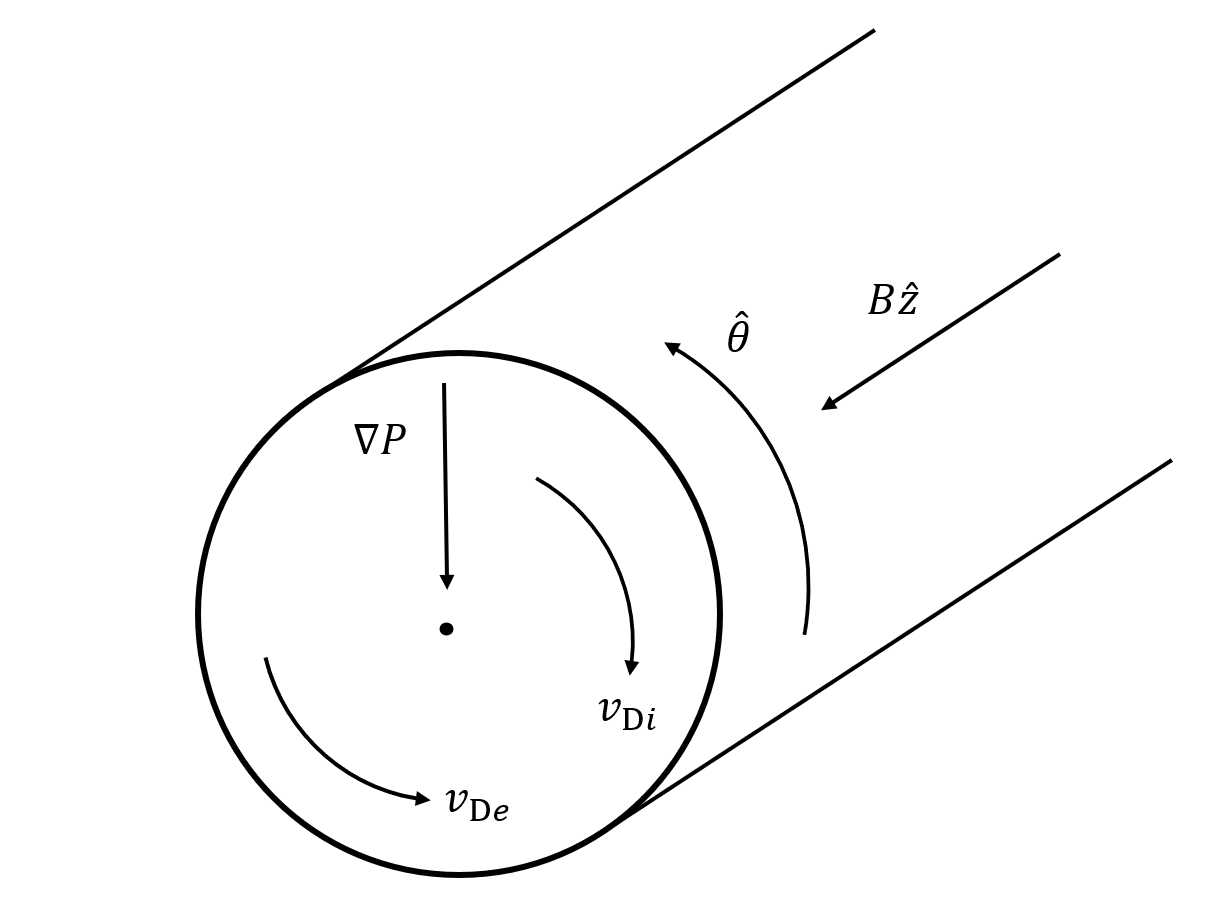
\includegraphics[width=0.7\linewidth]{entyuu_plasma.png}
	\caption{円柱プラズマ内の反磁性ドリフト}
	\label{fig:entyu}
\end{figure}
$\grad{P}\propto -\hat{r},\,\bm{B}\propto \hat{z}$であるため、$\bm{v}_{\text{D}}\propto -\hat{\theta}$となる。
すなわち、イオンの反磁性ドリフト、電子の反磁性ドリフトそれぞれが外部磁場$\bm{B}$を打ち消す方向の円電流を生むことがわかる。
そのため、プラズマ内に同じ方向の電流$\bm{j}_{\text{D}}$が生じることがわかる。その値はプラズマ近似$n_i=n_e=n$の元で
\begin{equation}
	\bm{j}_{\text{D}} = qn(\bm{v}_{\text{D}i} - \bm{v}_{\text{D}e}) = \qty(k_{\text{B}}T_i + k_{\text{B}}T_e)\frac{\bm{B}\cross\grad{n}}{B^2}
\end{equation}
である。
最後に、対流項が磁場に垂直な成分を持たないことを示す。
\begin{equation}
	\bm{v}\vdot\grad =
	\begin{pmatrix}
		v_r & v_\theta & v_z
	\end{pmatrix}
	\begin{pmatrix}
		\pdv{r}                 \\
		\frac{1}{r}\pdv{\theta} \\
		\pdv{z}
	\end{pmatrix}
\end{equation}
であることと、$\bm{v}_{\text{D}} = v(r)\hat{\theta}$と表されることより、
\begin{equation}
	\qty(\bm{v}_{\text{D}}\vdot\grad)\bm{v}_{\text{D}} = \qty(v(r)\frac{1}{r}\pdv{\theta})v(r)\hat{\theta} = 0
\end{equation}
となる。

\subsubsection{外部磁場に平行な流体ドリフト}
流体の運動方程式の$z$成分は
\begin{equation}
	mn\qty[\pdv{v_z}{t} + (\bm{v}\vdot\grad)v_z] = qnE_z - \pdv{p}{z}
\end{equation}
である。対流項は時間微分項に比べて無視できることが多い。$p=Cn^\gamma$を代入すると、
\begin{equation}
	\pdv{v_z}{t} = \frac{qE_z}{m} - \frac{\gamma k_{\text{B}}T}{mn}\pdv{n}{z}
\end{equation}
となる。$m\to 0$の極限(イオンに比べて電子の方が質量が小さいため、電子に対する運動方程式を考えていることになる。)をとると、
\begin{equation}
	qE_z = \frac{\gamma{}k_{\text{B}}T}{n}\pdv{n}{z}
\end{equation}
となる。$q=-e,\,\bm{E} = -\grad{\phi}$を用いて両辺を積分すると、
\begin{equation}
	n=n_0\exp\qty(\frac{e\phi}{k_{\text{B}}T})
\end{equation}
と求まる。すなわち、プラズマ中の電子(外部磁場に平行な成分)はBoltzmann分布をしていることになる。
イオンに比べて電子の質量は非常に小さいため、電子は大きな移動度を持つ。
電場によって速やかに高エネルギーに加速されるため、このような分布を取る。

\subsection{プラズマ近似}
電子の慣性項が無視できるとき、電子運動は低周波でなければならない。
逆に、高周波の運動を考える際には電子の慣性項が無視できなくなる:$m_e\pdv{\bm{v}_e}{t} \neq 0\;。$

電子が低周波運動を行っているとき、プラズマでは普通$n_i = n_e,\,\div{\bm{E}} \neq 0$を同時に満たされると仮定することが可能である。これをプラズマ近似と呼ぶ。
プラズマ近似が成立している際に$\bm{E}$を求めるためにPoisson方程式
\begin{equation}
	\div{\bm{E}} = 4\pi e(n_i-n_e)
\end{equation}
を用いることができないことに注意する必要がある。
また、電子が高周波で運動している場合にプラズマ近似ができないのは、イオンの質量が大きいため電子の運動に追従することができなくなり、電子とイオンの密度に差が生じてしまうからである。

\newpage
\section{方程式の線形化と単一モード解析}
いろんな種類の波に対する共通の考え方が方程式の線形化と単一モード解析である。
単一モード解析とは、各周波数$\omega$と波数$k$を用いて、物理量$\bm{A}$が
\begin{equation}
	\bm{A}(\bm{r},\,t) = \exp\qty{i\qty(\bm{k}\vdot\bm{r} - \omega{}t)}
\end{equation}
と表されることを元にして分散関係を導出することである。
方程式の線形化とは、全ての物理量を平衡成分と摂動成分(それぞれ添え字に0と1を)に分けることである。
そして、その摂動成分がどのような関数系になっているかを導出するということである。
また、摂動成分はその1次項までで近似する。
\subsection{プラズマ振動}
例として、電子に対する方程式群
\begin{gather}
	mn_e\qty[\pdv{\bm{v}_e}{t} + \qty(\bm{v}_e\vdot\grad)\bm{v}_e]  = -en_e\bm{E} \\
	\pdv{n_e}{t} + \div(n_e\bm{v}_e)                                = 0           \\
	\div{\bm{E}}                                                    = -4\pi{}en_e
\end{gather}
を線形化してみる。これは、プラズマ中の電子がイオンの一様なバックグラウンドから変位したときに、電子自身が生む電場によって元の位置に戻す復元力が働く場合を考えている。
すなわち、プラズマの中性を保とうとする方向の電場が自動的に生じている。これを解くと、電子は{\color{red}プラズマ周波数}と呼ばれる特性周波数で平衡位置を行き来して振動する。
その振動は非常に早く、イオンは電子の振動に追従できずに動かないと考える。最も簡単な場合として、
\begin{itemize}
	\item 外部磁場は存在しない。
	\item 熱運動はしていない。
	\item イオンは空間中に一様に分布し固定されている。
	\item プラズマは無限に大きい。
	\item 電子の運動は$\hat{\bm{x}}$方向のみである。
\end{itemize}
という仮定をおいて考える。
$\bm{E} = \bm{E}_0 + \bm{E}_1$として、$\bm{E}_1$成分について線形化すると、
\begin{gather}
	m\pdv{\bm{v}_1}{t}                                                    = -e\bm{E}_1 \\
	\pdv{n_{e1}}{t} + n_{e0}\div{\bm{v}_{e1}} + \bm{v}_{e0}\grad{n_{e0}}  = 0          \\
	\div{\bm{E}_1} = -4\pi e n_{e1}
\end{gather}
と1次の摂動で書ける。すべての摂動を$\exp\qty{i(\bm{k}\vdot\bm{r} - \omega{}t)}$として、
$\bm{v}_{e1} = v_1\hat{\bm{x}},\,\bm{E}_1 = E_1\hat{\bm{x}}$として解くと、線形化した方程式は
\begin{align}
	-im\omega{}v_1   & = -eE_1           \label{eq:1} \\
	-i\omega{}n_{e1} & = -n_{e0}ikv_{e1} \label{eq:2} \\
	ikE_1            & = -4\pi{}en_{e1} \label{eq:3}
\end{align}
となる。これはイオンについても同様に成立する。上の2式から
\begin{equation}
	n_{e1} = \frac{k}{\omega}n_{e0}v_{e1} = \frac{k}{\omega}n_{e0}\qty(\frac{-ie}{m\omega})E_1
\end{equation}
となり、これを最後の式に代入すると、
\begin{equation}
	\omega^2 E_1 = \frac{4\pi{}n_{e0}e^2}{m}E_1
\end{equation}
となり、
\begin{equation}
	\omega_{pe} = \sqrt{\frac{4\pi{}n_{e0}e^2}{m}}
\end{equation}
を電子プラズマ周波数と呼ぶ。質量$M$のイオンの寄与まで考えると、
\begin{equation}
	\omega^2E_1 =  4\pi{}n_{e0}e^2\qty(\frac{1}{m} + \frac{1}{M})E_1
\end{equation}
となり、
\begin{equation}
	\omega_{pi} = \sqrt{\frac{4\pi{}n_{e0}e^2}{M}}
\end{equation}
をイオンプラズマ周波数と呼ぶ。

\section{縦波}
\subsection{電子プラズマ波}
電子のプラズマ振動が熱運動によって伝播する波が電子プラズマ波である。熱運動を考慮するために断熱変化による圧力項
\begin{equation}
	P_e = C\rho_e^\gamma,\gamma=3
\end{equation}
を付与する。(一次元運動を考えるため$\gamma=3$となる。)このとき、両辺の対数微分と状態方程式$P_e = n_ek_{\text{B}}T_e$を用いると
\begin{equation}
	\grad{P_e} = 3k_{\text{B}}T_e\grad{n_e} = 3k_{\text{B}}T_e\grad(n_{e0} + n_{e1}) = 3k_{\text{B}}T_e\pdv{n_{e1}}{x}\hat{\bm{x}}
\end{equation}
となる。したがって、線運動方程式
\begin{equation}
	mn_e\pdv{\bm{v}_e}{t}= -en_e\bm{E} - \grad{P_e}
\end{equation}
を線形化すると、$x$方向は
\begin{equation}
	mn_{e0}\pdv{v_1}{t} = -en_{e0}E_1 - 3k_{\text{B}}T_e\pdv{n_{e1}}{x}
\end{equation}
となる。\footnote{摂動の2次以上の項は無視している。}
単一モード解析を行うと、式\eqref{eq:1}、式\eqref{eq:2}、式\eqref{eq:3}と同じようにして
\begin{align}
	-im\omega{}n_{e0}v_1 & = -en_0E_1  -3k_{\text{B}}T_eikn_{e1} \\
	-i\omega{}n_{e1}     & = -n_{e0}ikv_{e1}                     \\
	ikE_1                & = -4\pi{}en_{e1}
\end{align}
を組み合わせる。$n_{e1} = (k/{\omega})n_{e0}v_1$
を用いながら下2式を一番上の式に代入して、
\begin{equation}
	im\omega{}n_{e0}v_1  = en_{e0}i\frac{4\pi{}e}{k}\frac{k}{\omega}n_{e0}v_1 + 3k_{\text{B}}T_eik\frac{k}{\omega}n_{e0}v_1
\end{equation}
つまり、
\begin{equation}
	\omega^2v_1 = \qty(\frac{4\pi{}n_{e0}e^2}{m} + \frac{3k_{\text{B}}T_e}{m}k^2)v_1
\end{equation}
を得る。熱速度$v_{\text{th}}^2$を$v_{\text{th}}^2 = 2k_{\text{B}}T_e/m$で定義すると、分散関係は以下のようになる:
\begin{equation}
	\omega^2 = \omega^2_{pe} + \frac{3}{2}k^2v^2_{\text{th}}\;。
\end{equation}

電子プラズマ波の位相速度と群速度は
\begin{align}
	\text{位相速度}\quad{}v^2_{\phi} & \coloneqq \frac{\omega^2}{k^2} = \qty(\frac{\omega_{pe}}{k})^2 + \frac{3}{2}v^2_{\text{th}} \to \frac{3}{2}v^2_{\text{th}}\quad(k\to\infty)\;, \\
	\text{群速度}\quad{}v_g         & \coloneqq \pdv{\omega}{k} = \frac{c^2k}{\sqrt{\omega^2_{pe} + c^2k^2}} = \frac{c^2}{v_{\phi}} < c \quad\text{(情報の伝達速度)}\;,                     \\
\end{align}






\subsection{イオン音波}
\subsection{高域混成振動}
\subsection{低域混成振動}
\subsection{静電イオンサイクロトロン波}

\newpage
\section{横波}
\subsection{外部磁場がない場合}
$\bm{B}=\bm{0}$のときの横波であるため、$\bm{j}_1$をプラズマ電流として、Maxwell方程式から導かれる以下の方程式を解く:
\begin{align}
	\curl(\curl{\bm{E}}_1)   & =  \grad(\div{\bm{E}}_1) - \laplacian\bm{E}_1 = -\curl\dot{\bm{B}}_1\;, \\
	c^2\curl{\dot{\bm{B}}_1} & = 4\pi\pdv{\bm{j}_1}{t} + \ddot{\bm{E}}_1\;。
\end{align}
単一モード解析を用いると、横波では$\div{\bm{E}}_1 = \bm{k}\vdot\bm{E}_1 = 0$であることより
\begin{equation}
	c^2k^2\bm{E}_1 = -\qty(-4\pi{}i\omega{}\bm{j}_1 - \omega^2\bm{E}_1) \iff (\omega^2 - c^2k^2)\bm{E}_1 = -4\pi{}i\omega\bm{j}_1
\end{equation}
となる。なお、今の状況では以下の仮定を置いている:
\begin{itemize}
	\item 高周波振動を考えている。(イオンは不動である。)
	\item 電子の熱運動は考えていない。($\grad{P}$が発生して縦波を考えてしまうことになるため。)
\end{itemize}

プラズマ電子電流と電子の運動方程式はそれぞれ
\begin{align}
	\bm{j}_1              & = -n_0e\bm{v}_{e1}                                  \\
	m\pdv{\bm{v}_{e1}}{t} & = -e\bm{E}_1 \iff -im\omega\bm{v}_{e1} = -e\bm{E}_1
\end{align}
より
\begin{equation}
	\bm{j}_1 = \frac{in_0e^2}{m\omega}\bm{E}_1
\end{equation}
であるため、これを先ほどの式に代入すると、
\begin{equation}
	(\omega^2 - c^2k^2)\bm{E}_1 = \frac{4\pi n_0e^2}{m}\bm{E}_1 = \omega^2_{pe}\bm{E}_1 \iff \omega^2 = \omega^2_{pe} + c^2k^2
\end{equation}
と分散関係が求まる。位相速度、群速度、屈折率は以下のように計算される:
\begin{align}
	\text{位相速度}\quad{}v^2_{\phi} & \coloneqq \frac{\omega^2}{k^2} = c^2 + \frac{\omega^2_{pe}}{k^2} > c^2\;,                                                  \\
	\text{群速度}\quad{}v_g         & \coloneqq \pdv{\omega}{k} = \frac{c^2k}{\sqrt{\omega^2_{pe} + c^2k^2}} = \frac{c^2}{v_{\phi}} < c \quad\text{(情報の伝達速度)}\;, \\
	\text{屈折率}\quad{}N^2         & \coloneqq \frac{c^2}{v^2_{\phi}} = \frac{c^2k^2}{\omega^2} = 1 - \frac{\omega^2_{pe}}{\omega^2} < 1\;。
\end{align}
すなわち、プラズマ中では荷電粒子の塊が存在しているはずであるが、真空よりも屈折率が低いという奇妙な結果が生じている。また、以下のような事実がわかる:
\begin{itemize}
	\item プラズマの電子密度が大きくなると、$\omega_{pe}\propto \sqrt{n}$であるため屈折率は小さくなっていく。
	\item $\omega=\omega_{pe}$となるプラズマ密度$n_e = \frac{m\omega^2_{pe}}{4\pi e^2}$(臨界密度)で電磁波が遮断される。プラズマは$\omega > \omega_{pe}$を満たす高周波の波しか通さない。{\color{red}物理的にはなぜ?}
	      \begin{itemize}
		      \item 通信衛星を考えると、電離層に遮断されないように高周波帯域を用いる方が良い。
		      \item 地上での通信では電離層で反射させるために低周波帯域を用いる方が良い。
	      \end{itemize}
\end{itemize}
\subsection{正常波}
\subsection{異常波}
\subsection{外部磁場と波数ベクトルが平行な場合}

\end{document}